
\documentclass[ba, 11pt]{imsart}
%
%\pubyear{0000}
%\volume{00}
%\issue{0}
%\doi{0000}
%\arxiv{}
\firstpage{1}
\lastpage{1}

\usepackage{color}
\usepackage{float}
\usepackage{graphicx}
\usepackage{url}
\usepackage{natbib}
\usepackage[colorlinks,citecolor=blue,urlcolor=blue,filecolor=blue,backref=page]{hyperref}
\usepackage{mathtools, amsthm, bm}
\usepackage{subfig}
\usepackage{threeparttable, booktabs}
\usepackage{titling}
\usepackage{unicode-math}
\usepackage{wrapfig}
\usepackage{xcolor}
\usepackage{minted}
%\usepackage[notext]{stix2}
\setmathfont{STIX2Math.otf}

\usepackage{xeCJK}
  \xeCJKsetup{%
    CJKspace=true,% % true이면 띄어쓰기 사용. 중국어, 일어는 필요 없을수도
    % CJKmath=true,%  % true면 math environment 안에서 CJK 글자 사용
    CJKecglue={},%   % Western과 CJK 사이의 공백 지정: {}로 간격을 없앰
    BoldFont={NanumgothicB.ttf}
  }
\setCJKmainfont{NanumGothic.ttf}
\setCJKsansfont{NanumGothic.ttf}
\setCJKmonofont{NanumGothic.ttf}

\newcommand{\va}{\mathbf{a}}
\newcommand{\vb}{\mathbf{b}}
\newcommand{\vc}{\mathbf{c}}
\newcommand{\vd}{\mathbf{d}}
\newcommand{\ve}{\mathbf{e}}
\newcommand{\vf}{\mathbf{f}}
\newcommand{\vg}{\mathbf{g}}
\newcommand{\vh}{\mathbf{h}}
\newcommand{\vi}{\mathbf{i}}
\newcommand{\vj}{\mathbf{j}}
\newcommand{\vk}{\mathbf{k}}
\newcommand{\vl}{\mathbf{l}}
\newcommand{\vm}{\mathbf{m}}
\newcommand{\vn}{\mathbf{n}}
\newcommand{\vo}{\mathbf{o}}
\newcommand{\vp}{\mathbf{p}}
\newcommand{\vq}{\mathbf{q}}
\newcommand{\vr}{\mathbf{r}}
\newcommand{\vs}{\mathbf{s}}
\newcommand{\vt}{\mathbf{t}}
\newcommand{\vu}{\mathbf{u}}
\newcommand{\vv}{\mathbf{v}}
\newcommand{\vw}{\mathbf{w}}
\newcommand{\vx}{\mathbf{x}}
\newcommand{\vy}{\mathbf{y}}
\newcommand{\vz}{\mathbf{z}}
\newcommand{\valpha}{\pmb{\alpha}}
\newcommand{\vtheta}{\pmb{\theta}}

\newcommand{\mA}{\mathbf{A}}
\newcommand{\mB}{\mathbf{B}}
\newcommand{\mC}{\mathbf{C}}
\newcommand{\mD}{\mathbf{D}}
\newcommand{\mE}{\mathbf{E}}
\newcommand{\mF}{\mathbf{F}}
\newcommand{\mG}{\mathbf{G}}
\newcommand{\mH}{\mathbf{H}}
\newcommand{\mI}{\mathbf{I}}
\newcommand{\mJ}{\mathbf{J}}
\newcommand{\mK}{\mathbf{K}}
\newcommand{\mL}{\mathbf{L}}
\newcommand{\mM}{\mathbf{M}}
\newcommand{\mN}{\mathbf{N}}
\newcommand{\mO}{\mathbf{O}}
\newcommand{\mP}{\mathbf{P}}
\newcommand{\mQ}{\mathbf{Q}}
\newcommand{\mR}{\mathbf{R}}
\newcommand{\mS}{\mathbf{S}}
\newcommand{\mT}{\mathbf{T}}
\newcommand{\mU}{\mathbf{U}}
\newcommand{\mV}{\mathbf{V}}
\newcommand{\mW}{\mathbf{W}}
\newcommand{\mX}{\mathbf{X}}
\newcommand{\mY}{\mathbf{Y}}
\newcommand{\mZ}{\mathbf{Z}}

\newtheorem{theorem}{\textbf{Theorem}}
\newtheorem{definition}{\textbf{Definition}}
\newtheorem{proposition}{\textbf{Proposition}}

\DeclareMathOperator*{\minimize}{minimize}
\DeclareMathOperator*{\maximize}{maximize}
\DeclareMathOperator*{\argmax}{arg\,max}
\DeclareMathOperator*{\argmin}{arg\,min} 

\startlocaldefs
% ** Local definitions **
\endlocaldefs

\begin{document}

%% *** Frontmatter *** 

\begin{frontmatter}
  \title{가우시안 프로세스와 인구조사 데이터를 이용한 \\ 캘리포니아 지역 주택 가격 예측}

%\title{\thanksref{T1}}
%\thankstext{T1}{<thanks text>}
\runtitle{}

\begin{aug}
  \author{20161453 전자공학과\\김규래}%\textsuperscript{*}}
  \address{}
%\author{\fnms{<firstname>} \snm{<surname>}\thanksref{}\ead[label=e1]{}}
%\and
%\author{\fnms{} \snm{}}

%\runauthor{}

\end{aug}


%\begin{abstract}
%\end{abstract}

%% ** Keywords **
%\begin{keyword}%[class=MSC]
%\kwd{}
%\kwd[]{}
%\end{keyword}

\end{frontmatter}

\section{Introduction}\label{}
이 프로젝트에서는 캘리포니아의 인구조사 데이터를 이용해서 주택의 가격을 예측하는 모델을 만들어본다.
예측을 위해서는 Gaussian process (GP) regression~\citep{rasmussen_gaussian_2006} 머신러닝 방식을 사용하였다.
GP는 kernel method와 Bayesian machine learning을 접목한 머신러닝 알고리즘으로, feature transformation을 특별히 하지 않아도 굉장히 좋은 성능을 내는 방식이다.
이론적으로는 딥러닝과 매우 깊은 관계를 갖고 있다.
다만, GP는 계산량이 많다는 이유로 최근에는 더 scalable한 딥러닝 방식에 밀리는 편이다.
이번 프로젝트에서는 캘리포니아 인구 조사 데이터에 GP를 적용해서 deep learning 방식인 multi-layer perceptron (MLP)와 성능이 얼마나 차이가 나는지를 알아보는 것을 목표로 한다.

보고서의 기본 구조는 다음과 같다.
Section~\ref{section:anal}에서는 먼저 데이터셋의 간단한 분석을 진행하였고, Section~\ref{section:method}에 GP에 대한 간단한 소개와 구현한 방식을 서술하였다.
마지막으로, Section~\ref{section:eval}에 구현한 GP 모델의 성능을 평가하였다.

이번 과제에서는 다음의 것들을 직접 구현하였다.
\begin{itemize}
  \item Gaussian process regression 알고리즘을 Julia 언어~\citep{bezanson_julia_2017}를 이용해서 직접 구현하였다.
  \item Elliptical slice sampling 알고리즘을 Julia 언어로 직접 구현하였다.
  \item 비교를 위한 multi-layer perceptron을 Julia의 deep learning 라이브러리, \textsc{Flux}.jl를 이용해서 구현하였다.
\end{itemize}

구현한 코드는 Julia 언어를 설치한 후, 다음과 같이 실행할 수가 있다.
\definecolor{bg}{rgb}{0.85,0.85,0.85}
\begin{minted}[autogobble,
    bgcolor=bg,
    framesep=2mm,
    baselinestretch=1,
    breaklines]{julia}
  ] add CUDA, Distributions, KernelFunctions, LinearAlgebra, ProgressMeter, Random, DelimitedFiles, XLSX, DataFrames, DataFramesMeta
    include("gp.jl");
    main(:train); # Training 
    main(:test)   # Test
\end{minted}

\section{Dataset Analysis}\label{section:anal}
먼저, 예측 방법론을 선택하기 이전에 주어진 데이터셋을 분석하였다. 
주어진 데이터셋은 미국 california (CA) 지역의 주택 정보와 주택의 가격을 정리한 데이터셋이다.
기본적으로 Table~\ref{table:features}과 같은 feature들로 이루어져 있고, 이 feature들을 이용해서 주택의 가격을 예측하는 것을 목표로 한다.
%
\begin{table*}
  \centering
  \begin{threeparttable}
    \caption{Dataset의 Feature들의 특성}\label{table:features}
    \begin{tabular}{cllrr} \toprule
      \textbf{Index}
      & \multicolumn{1}{c}{\textbf{Feature}}
      & \multicolumn{1}{c}{\textbf{Continuity}}
      & \multicolumn{1}{c}{\textbf{Min.}}
      & \multicolumn{1}{c}{\textbf{Max.}}
      \\ \midrule
      1 & Longitude           & Continuous & -124 & -114 \\
      2 & Latitude            & Continuous & 32  & 42 \\
      3 & Housing median age  & Continuous & 0   & 1000 \\
      4 & \# of Rooms         & Continuous & 1   & 100 \\
      5 & \# of bedrooms      & Continuous & 1   & 100 \\
      6 & Population          & Continuous & 10  & \(40 \times 10^6\) \\
      7 & Households          & Continuous & 0   & \(10 \times 10^6\) \\
      8 & Median income (\$, \(10^3\)) & Continuous & 0   & 100 \\
      9 & Ocean proximity     & Categorial & 1 & 4 \\\bottomrule
    \end{tabular}
  \end{threeparttable}
\end{table*}

\paragraph{Feature들의 연속성}
먼저, feature들의 연속성을 간단하게 분석해서 Table~\ref{table:features}에 정리하였다.
연속성은 머신러닝 모델을 선택할 때 매우 중요한 정보이다.
특히 regression의 경우, 연속성을 고려할 수 있느냐 없느냐에 따라 다른 접근들을 사용해야 한다.
주어진 CA 데이터셋의 경우, \textit{Ocean proximity}를 제외하고서는 모든 feature들이 연속성을 가진다.
Ocean proximity의 경우 약하게 continuity를 보인다고 생각할 수도 있겠으나, 일단 Categorical로 분류를 하였다.

\paragraph{Feature 값들의 범위}
머신러닝 모델에 따라서는 feature들의 값을 제안하거나 일정한 범위로 normalization을 해줘야하는 경우들이 많다.
따라서, 각 feature들의 최댓값과 최솟값을 분석해서 Table~\ref{table:features}에 정리하였는데, 이 최댓값과 최솟값에 대한 가정들은 데이터셋을 관찰하지 않은 사전 가정(prior information)으로 두기 위해서 데이터셋의 값들을 이용하지 않았다.
첫째로, \textit{longitude}와 \textit{latitude}는 CA 지역의 실제 longitude와 latitude 범위를 인터넷으로 조사해서 설정하였다.
\textit{Housing median age}의 최대값의 경우, 특별한 가정을 설정하지 않고 미국이 존재한 기간보다 훨씬 오래전인 1000년으로 설정하였다.
\textit{\# of Rooms}와 \textit{\# of bedrooms} 또한 특별한 가정 없이 100 정도로 설정하였다.
\textit{Population}은 CA의 2019년 전체 인구를 반올림한 값인 40M으로 설정하였다.
비슷하게, 4인 가정을 가정할 때 전체 인구로부터 유추할 수 있는 가정의 갯수 10M를 \textit{Households}의 최댓값으로 설정하였다.
\textit{Median income}의 최대값은 \$1M로 설정하였다.
마지막으로, \textit{Ocean proximity}는 각 값에 1\~4 사이 임의의 값을 지정하였다.

\paragraph{Feature들의 경향 분석}
사용할 모델을 선택하기 위해서는 feature들의 경향을 분석해서 적절한 feature transformation을 적용하는 것이 매우 중요하다.
이를 위해서, train-test set을 미리 분리한 다음, train set의 feature들을 Figure~\ref{fig:feature} 시각화하였다.
먼저, feature들의 선형성을 살펴보면, \textit{median income}을 제외하고 전반적으로 feature들이 선형성을 보이지 않는 것을 볼 수 있다.
특히, \textit{housing median age}를 보면 target과 feature간의 correlation이 거의 없는 것을 알 수가 있다.
longitude와 latitude의 경우, 선형성은 보이지 않지만 data point간의 cluster들이 형성되는 것을 확인할 수 있다.
\textit{\# of rooms}, \textit{\# of bedrooms}, \textit{population}을 보면, log-scale로 변환할 경우 target과 feature간의 약한 correlation이 보이나, variance가 굉장히 큰 것을 알 수가 있다.
전반적으로 볼 때, 어떠한 feature transform을 적용한다고 해서 feature와 target간의 관계가 명확하게 개선될 것을 기대하기가 어렵다고 판단하였다.

\paragraph{Feature간의 correlation}
마지막으로, Figure~\ref{fig:feqture_corr}를 보면 feature간의 correlation을 시각화한 것을 볼 수 있다.
이를 보면 4\~7번 feature와 1\~2번 feature들이 매우 강한 correlation을 띄고 있는 것을 알 수가 있는데, 이 때문에 feature간의 independence를 이용하는 머신러닝 모델은 사용하지 않는 것이 좋을 것으로 예상할 수 있다.


    %% # 114 < longitude           < 124,    Δ = 10
    %% # 32  < latitude            < 42,     Δ = 10
    %% # 0   < housing_median_age  < 1000,   Δ = 1000
    %% # 1   < total_rooms         < 100,    Δ = 99
    %% # 1   < total_bedrooms      < 100,    Δ = 99
    %% # 10  < population          < 40e+6,  Δ ≈ 40e+6
    %% # 0   < households          < 10e+6,  Δ ≈ 10e+6
    %% # 0   < median_income (10k) < 100,    Δ = 100
    %% # 1   < ocean_proximity     < 4,      Δ = 3


\begin{figure*}
  \centering
  \subfloat[Longitude]{
    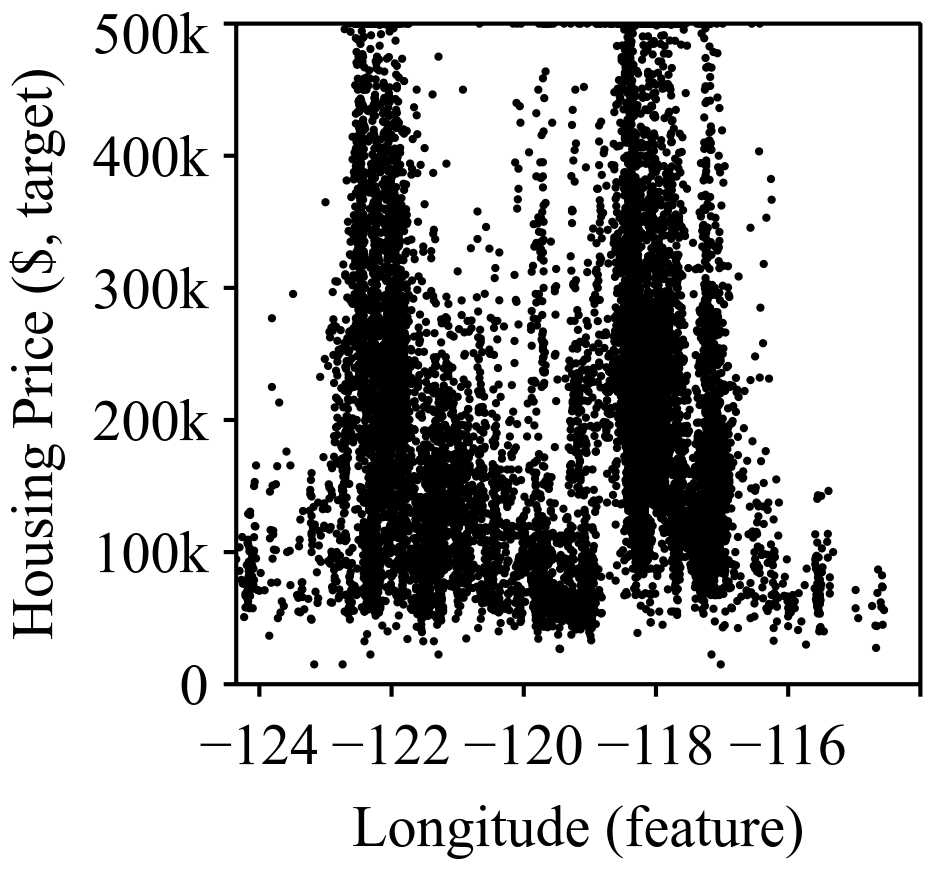
\includegraphics[scale=0.5]{figures/feature_viz_01.png}
  }
  \subfloat[Latitude]{
    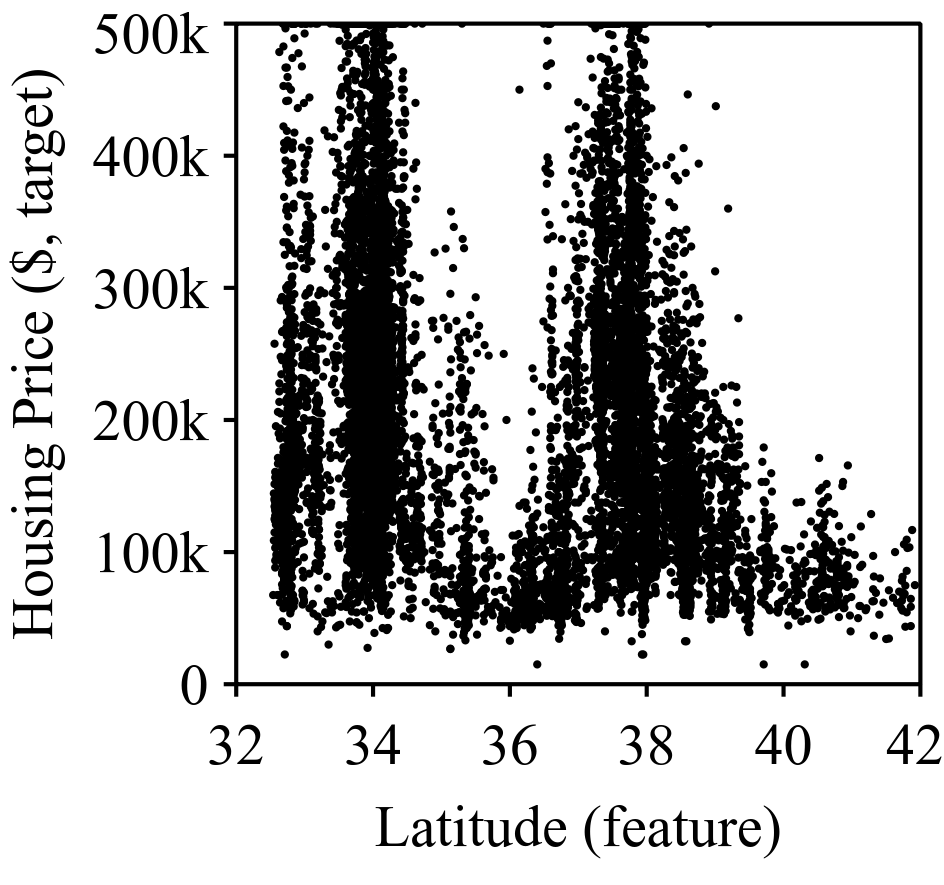
\includegraphics[scale=0.5]{figures/feature_viz_02.png}
  }
  \subfloat[Housing median age]{
    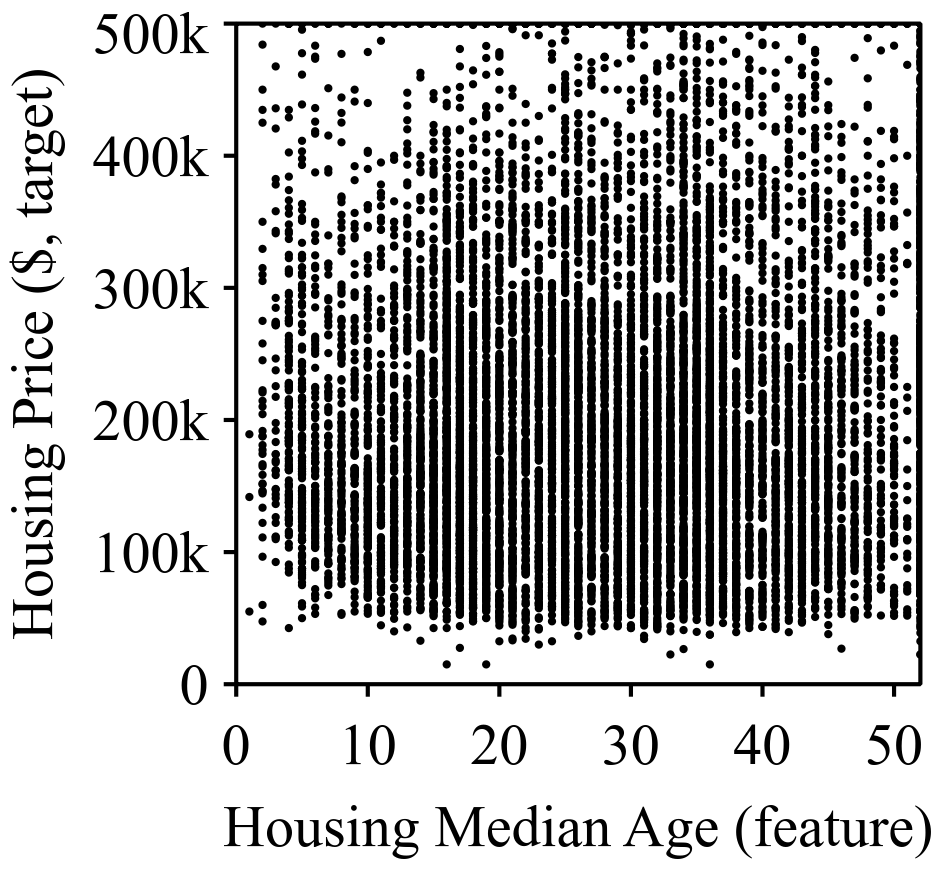
\includegraphics[scale=0.5]{figures/feature_viz_03.png}
  } \\
  \subfloat[\# of rooms]{
    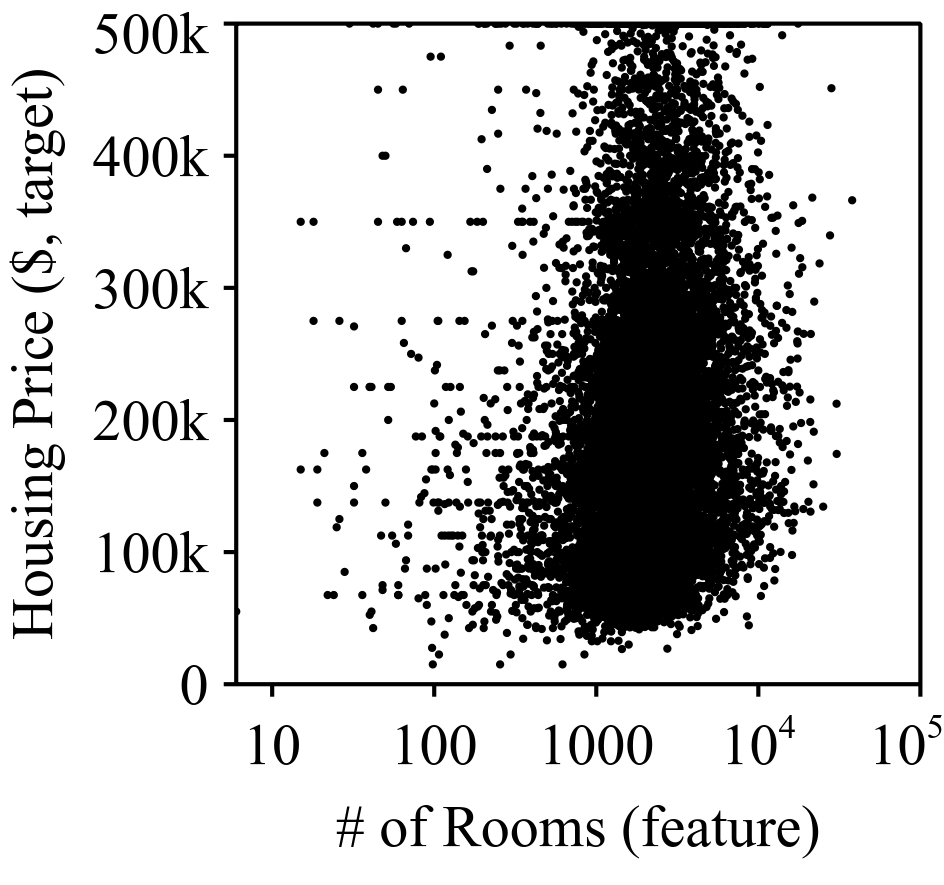
\includegraphics[scale=0.5]{figures/feature_viz_04.png}
  }
  \subfloat[\# of bedrooms]{
    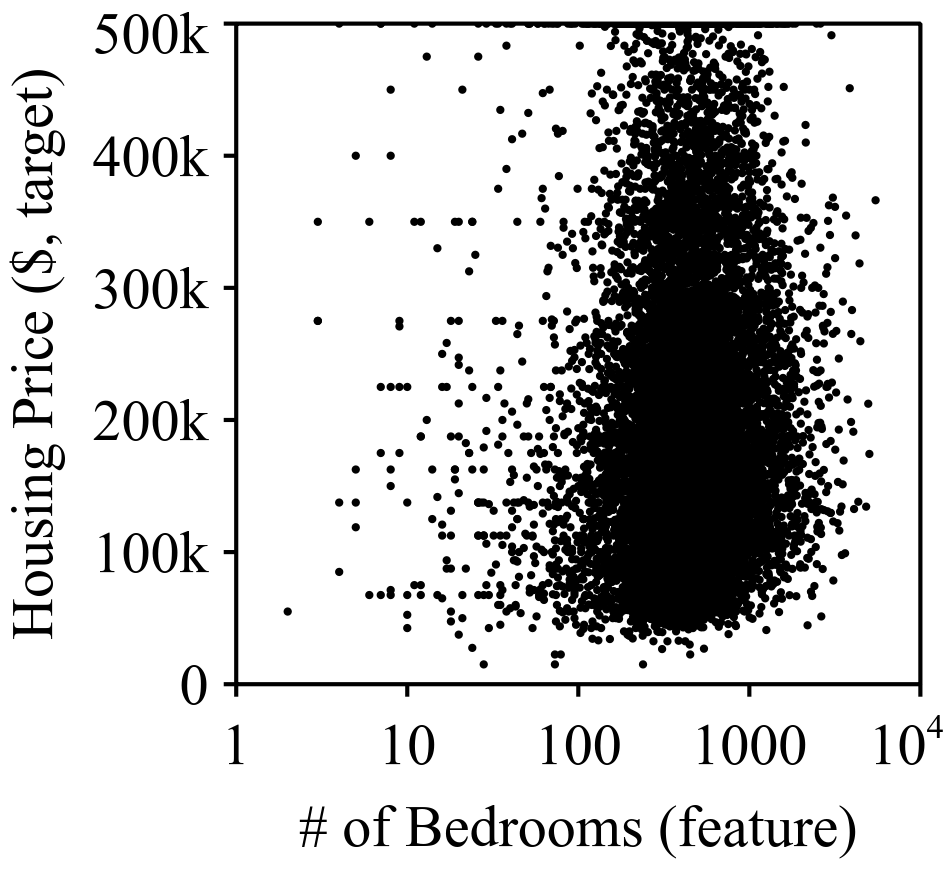
\includegraphics[scale=0.5]{figures/feature_viz_05.png}
  }
  \subfloat[Population]{
    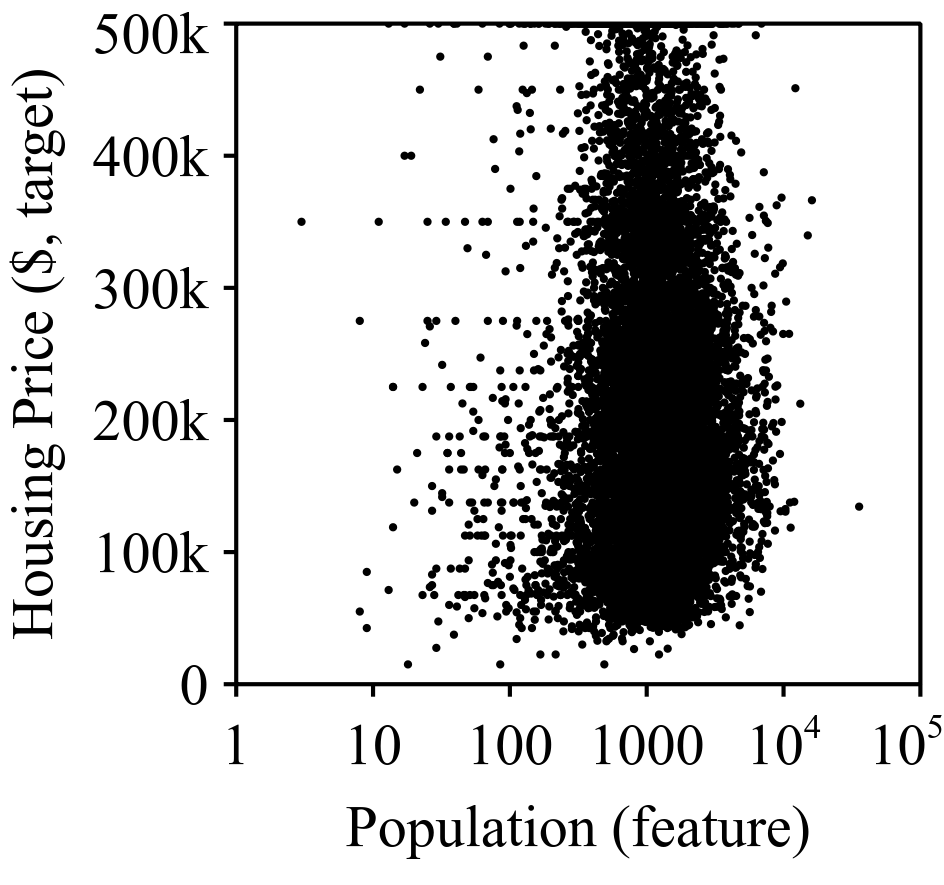
\includegraphics[scale=0.5]{figures/feature_viz_06.png}
  } \\
  \subfloat[Households]{
    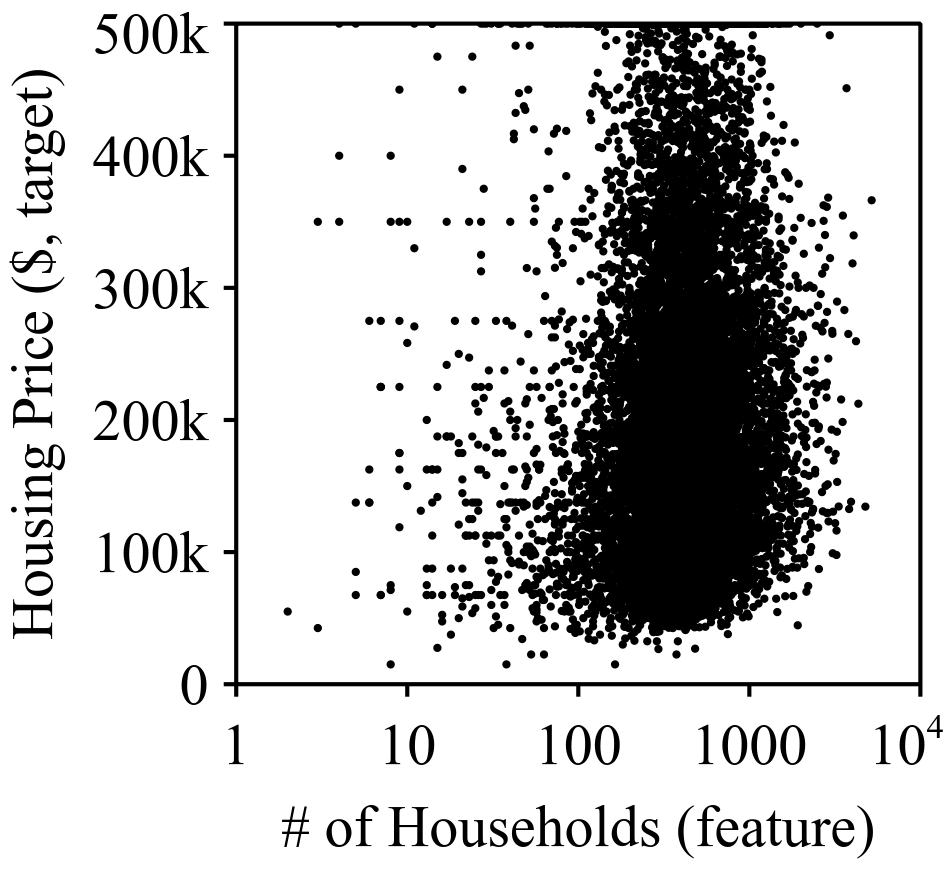
\includegraphics[scale=0.5]{figures/feature_viz_07.png}
  }
  \subfloat[Median income]{
    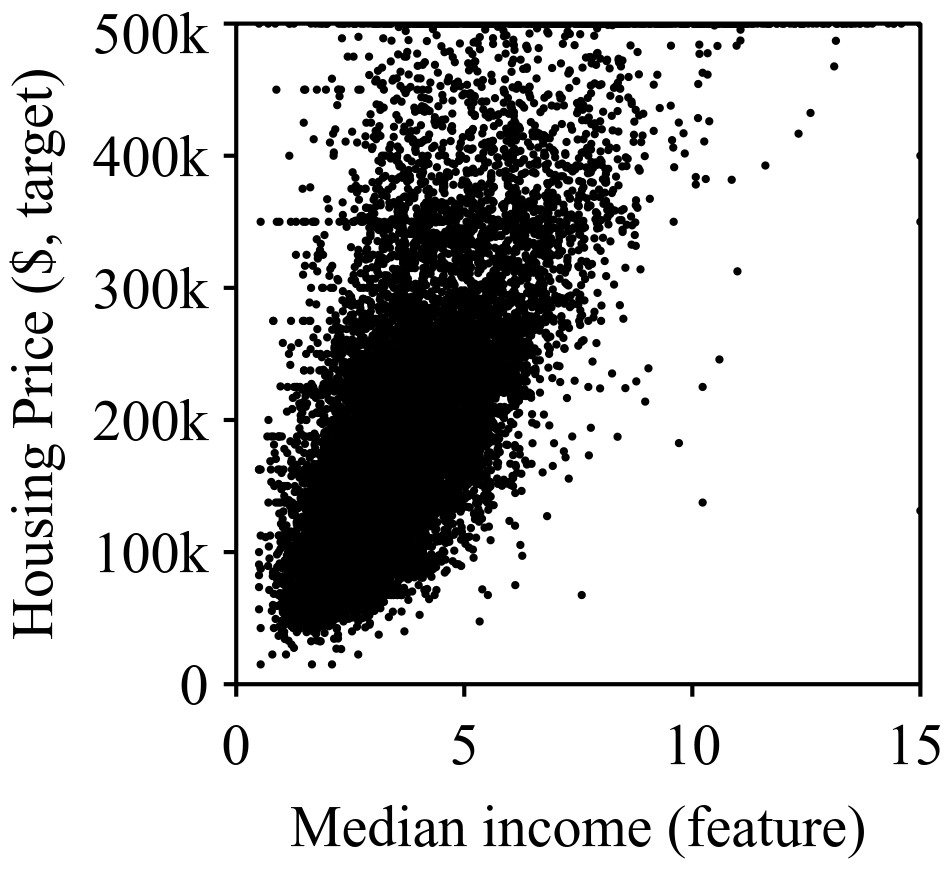
\includegraphics[scale=0.5]{figures/feature_viz_08.png}
  }
  \subfloat[Correlation Matrix]{
    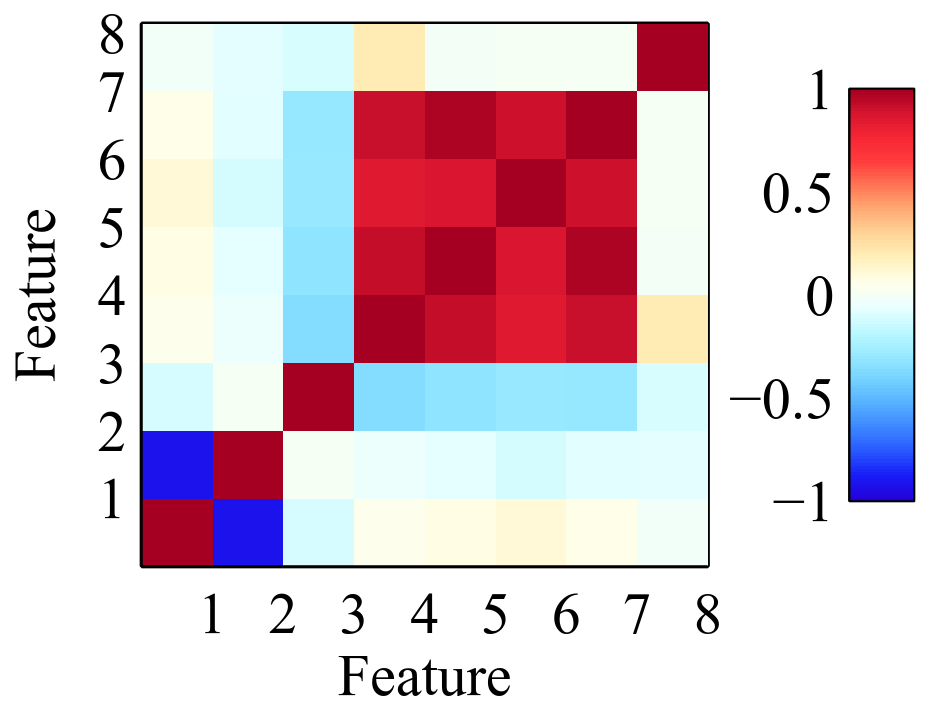
\includegraphics[scale=0.6]{figures/feature_viz_09.png}\label{fig:feqture_corr}
  }
  \caption{CA dataset의 feature들의 시각화.}\label{fig:feature}
\end{figure*}

\paragraph{분석 결론}
Dataset의 특성들을 분석한 결과로부터 얻은 결론들은 다음과 같다.
\begin{itemize}
  \item Feature들이 전반적으로 target variable과 선형성이 떨어진다.
  \item Feature들간의 correlation이 상당히 높다.
  \item Cluster관계를 보이는 feature들이 일부 있다.
  \item Log-scale로 변환하는 것이 좋은 feature들이 일부 있다.
\end{itemize}
문제는, 이 사실들을 전부 적절하게 사용할 수 있는 feature transformation이 많지 않다는 점이다.
따라서, feature transformation을 직접 해주지 않아도 feature들을 적절히 학습을 할 수 있는 머신러닝 모델을 활용하였다.
이러한 머신러닝 모델로는 kernel method들이 대표적인데, 그 중에서도 regression에 특화된 모델인 Gaussian process regression을 사용하였다.


\section{Methodology}\label{section:method}
\subsection{Gaussian Processes}\label{section:gp}
\paragraph{Kernel linear regression}
Gaussian processes (GP) 는 kernel linear regression을 Bayesian방식으로 해석한 모델이다.
kernel linear regression은 
\begin{align}
  f(\vx) = \langle \vw, \phi(\vx) \rangle, \;\;\; \phi : \mathcal{X} \rightarrow \mathcal{H}
\end{align}
와 같이 정의가 되는 regression 모델이다.
feature space에 있는 \(\vx \in \mathcal{X}\)를 어떠한 latent space \(\mathcal{H}\)로 보내는 feature transform \(\phi\)를 활용하는 방법이다.
이 때 \(\mathcal{H}\)는 사용하는 kernel \(k(\cdot, \cdot)\)에 의해 정의되는 reproducing-kernel Hilbert space이다.
이 프로젝트에서 사용한 \(k\)의 경우, 무한한 차원을 가지는 \(\mathcal{H}\)를 생성한다.

\paragraph{Gaussian Processes}
위의 kernel linear regression 모델에다가
\begin{align}
  p(y \,|\, \vw, \vx) &= \mathcal{N}(f(\vx); y, \sigma^2_{\mathcal{\epsilon}}) \\
  p(\vw)              &= \mathcal{N}(\vw; \mu, \Sigma)
\end{align}
와 같이 likelihood (\(p(y \,|\, \vw, \vx)\))와 prior (\(p(w)\))를 정의하면, Gaussian process가 된다.
이를 probabilistic graphical model로 해석하는 경우, 
\begin{align}
  \theta                        &\sim \mathcal{N}(\,0, \sigma^2_{\epsilon}\,) \\
  \vf \,|\, \mathcal{D}, \theta &\sim \mathcal{N}(\, \mu_{\vf \,|\, \mathcal{D}, \theta}, \Sigma_{\vf \,|\, \mathcal{D}, \theta}\,) \\
  y   \,|\, \vf, \vx            &\sim \mathcal{N}(\, \mu(\vx), \sigma^2(\vw)\,)
\end{align}
와 같이 표현이 되고, predictive distribution은
\begin{align}
 \mu(\vx)      &= {\vk(\vx)}^{\top } {(\mK + \sigma^2_{\epsilon} \mI)}^{-1} \vy \label{eq:mu} \\
 \sigma^2(\vx) &= k(\vx, \vx) - {\vk(\vx)}^{\top}{(\mK + \sigma^2_{\epsilon} \mI)}^{-1} {\vk(\vx)} \label{eq:sigma}
\end{align}
로 주어진다~\cite{rasmussen_gaussian_2006}.
여기서 \(k(\cdot, \cdot)\)은 두 점 간의 kernel function의 값으로, covariance라고 부르겠다.
\({[\vk(\cdot)]}_i = {k(\cdot, \vx_i)}, \; {\vx_i \in \mathcal{D}}\)는 dataset의 각 feature vector와의 covariance vector이고,
\({[\mK]}_{i,j} = {k(\vx_i, \vx_j)}, \; {\vx_i, \vx_j \in \mathcal{D}}\)는 dataset의 각 feature vector간의 covariance matrix이다.
\(\mK\)는 더 흔한 이름인 Gram matrix라고 부르겠다.
마지막으로, \({[\vy]}_{i} = y_i, \; y_i \in \mathcal{D} \)는 dataset의 target variable들을 전부 붙인 vector이다.

\paragraph{Marginal likelihood}
GP는 특이하게도, latent variable인 \(\vf\)가 closed-form으로 marginalization이 가능하다.
따라서, marginal likelihood를
\begin{align}
  p(\mathcal{D} | \theta) &= \int p(\mathcal{D} \,|\, \vf, \theta) \, p(\vf \,|\, \theta) \, p(\theta) \, d\vf \\
  &\propto \exp\Big(\;  \frac{1}{2} \vy^{\top} {(\mK + \sigma^2_{\epsilon} \mI)}^{-1} \vy - \frac{1}{2} \log{|\mathbf{K}|} - \frac{|\mathcal{D}|}{2} \log{2 \pi} \;\Big)
\end{align}
와 같이 구할 수가 있다.
이를 이용하면, hyperparameter \(\theta\)를 Bayesian inference를 이용해 추론할 수가 있다.

\paragraph{Kernel 선택}
GP regression을 할 때는 squared-exponential kernel이나 Matern kernel을 가장 많이 사용한다.
특히, 모델링하고자 하는 함수가 2번 미분 가능하다는 가정을 동반하는 Matern 5/2 kernel이 가장 많이 사용된다.
Matern kernel은
\begin{align}
  k(\vx_i, \vx_j) &= k_{\text{ARD}}( \vx_i^{\top} \Sigma^{-1}  \vx_j )\\
  k_{\text{ARD}}(\Delta \vx)  &= \sigma^2 \frac{2^{1 - \nu}}{\Gamma(\nu)} \big( \sqrt{2 \nu} \, \Delta\vx \big) \, K_\nu \big( \sqrt{2 \nu} \, \Delta \vx \big) \\
  \Sigma &= \text{Diagonal}([\, \ell_1^2, \ell_2^2, \ldots, \ell_N^2 \,])
\end{align}
로 주어지고, 이 때 \(\Gamma\)는 gamma 함수, \(K_\nu(\cdot)\)는 modified Bessel 함수이다.
이 때 \(\nu = 5/2\)를 흔히 사용하므로, 그렇게 설정하였다.
\(\Sigma\)의 경우, 위와 같이 diagonal matrix를 사용하는 경우를 automatic relevance determination (ARD)라고 부르는데, 주어진 dataset의 경우 feature마다 scale이 크게 차이가 나므로 ARD를 사용하였다.
\(\Sigma\)의 값들은 hyperparameter \(\theta\)에 포함시켜서 Bayesian inference로 추론하였다.

\paragraph{Hyperparameter 처리}
GP는 hyperparameter의 선택에 굉장히 민감한 것으로 알려져 있다~\citep{rasmussen_gaussian_2006}.
특히, noise variance \(\sigma^2_{\epsilon}\)과 ARD kernel의 length scale \(\ell_i^2\)가 결과에 많은 영향을 미친다.
이를 처리하는 방법은  
\begin{align}
  \vtheta^*_{\text{MAP-II}} &= \argmax_{\vtheta}\; p(\mathcal{D} \,|\, \vtheta) p(\vtheta) \\
  \mu(\vx) &\approx \mu(\vx;  \vtheta^*_{\text{MAP-II}})
\end{align}
형태로 maximum a-posteriori type 2 (MAP-II)를 수행하거나, 
\begin{align}
  \mu(\vx) = \int \mu(\vx \,|\, \vtheta) p(\vtheta \,|\, \mathcal{D}) d\vtheta\label{eq:hyper_marg}
\end{align}
형태로 marginalization을 하는 것이다.
일반적으로는 marginalization이 hyperparameter의 불확실성을 잘 고려하기 때문에 더 좋은 결과를 보이는 것으로 알려져 있다~\cite{murphy_machine_2012}.
또한, Gaussian process는 수치적 불안전성 때문에 MAP-II를 계산하는 것이 실패하는 경우들이 종종 있다.
Marginalization을 수행하기 위한 알고리즘들은 이러한 이슈들로부터 조금 더 자유롭다.

Marginalization은 수식~\eqref{eq:hyper_marg}의 적분을 계산할 수 있어야 하는데, 이는 많은 경우에 불가능하다.
GP의 hyperparameter의 경우에도 이 적분식을 계산할 수가 없다.
따라서 이를 
\begin{align}
  \int \mu(\vx \,|\, \vtheta) \, p(\vtheta \,|\, \mathcal{D}) \, d\vtheta \approx \frac{1}{N} \sum_{\vtheta_i \sim p(\theta_i \,|\, \mathcal{D})}^N \mu(\vx \,|\, \vtheta_i) \label{eq:mc}
\end{align}
형태로 Monte Carlo 근사를 수행해야 한다.

\subsection{Implementation}\label{}
\paragraph{Overview}
Section~\ref{section:gp} 에서 소개한 GP는 별도로 라이브러리를 사용하지 않고 직접 Julia 언어~\citep{bezanson_julia_2017}를 이용해서 구현하였다.
Julia언어는 MATLAB이나 Python과 같은 하이레벨 문법을 지원하면서도, Fortran이나 C++와 같은 언어들의 높은 성능을 이용할 수 있게 해준다.
또한, CUDA문법을 사용하지 않고 Julia언어의 문법만 사용하면서 CUDA 프로그래밍을 할 수 있게 해준다.
주어진 데이터셋의 경우, GP를 쓰기에는 상당히 큰 편이기 때문에 GP 라이브러리들 대신에 GPU를 활용할 수 있는 최적화된 코드를 직접 작성해서 training 기간을 줄일 수 있었다.

\paragraph{Gaussian Process 추론}
Gaussian process는 수식~\eqref{eq:mu},~\eqref{eq:sigma}에서 볼 수 있듯이, 역행렬을 한번 계산해야된다.
일반적으로는, 역행렬을 계산하는 대신 
\begin{align}
  \mu(\vx) &= {\vk(\vx)}^{\top } {(\mK + \sigma^2_{\epsilon} \mI)}^{-1} \vy \\
  &= {\vk(\vx)}^{\top } \valpha
\end{align}
형태로 \( \valpha = {(\mK + \sigma^2_{\epsilon} \mI)}^{-1} \vy \)를 미리 계산 해두는데, 이 과정을 GP training 이라고 부른다.
따라서, GP training 단계에서는 선형방정식을 한번 풀어야 하는데, dataset에서 data point의 갯수 \(N\)에 대해서 \(\mK \in \mathbb{R}^{N \times N}\) 이므로, \(N\)개의 변수를 가진 연립방정식이다.
\(\mK\)는 symmetric matrix이고, Gram matrix의 특성으로 인해 positive definite matrix이다.
고로, Cholesky decomposition과 back-substitution을 이용해서
\begin{align}
  \mL    &\leftarrow \text{Cholesky}(\mK + \sigma^2_{\epsilon} \mI) \\
  \alpha &\leftarrow \mL^\top \, \backslash \, \mL  \, \backslash \, \vy \label{eq:alpha}
\end{align}
와 같이 이 연립방정식을 푸는 것이 일반적이다~\citep{rasmussen_gaussian_2006}.
\(\backslash\)는 back-substitution을 의미한다.

\begin{figure}[t]
  \centering
  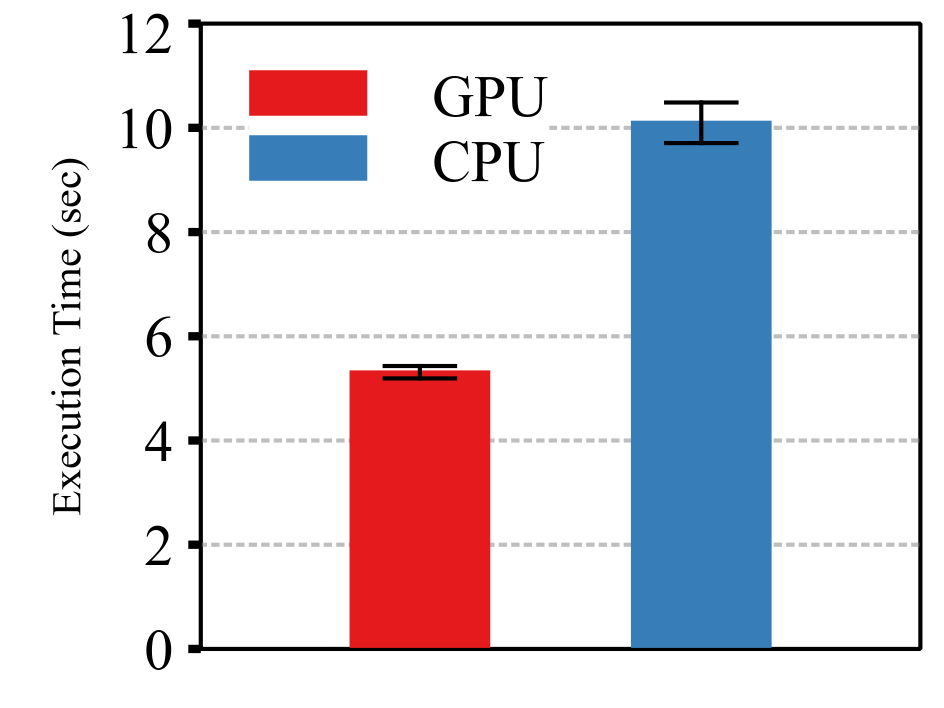
\includegraphics[scale=0.7]{figures/exectime_01.png}
  \caption{CPU와 GPU 계산 속도 비교.
    오차 범위는 실행시간을 8번 측정한 것의 10\%와 90\% quantile이다.}\label{fig:exec_time}
\end{figure}
%
\paragraph{GPU implementation}
주어진 CA 데이터셋의 경우 \(N=16k\) 정도이므로, CPU로 계산할 경우 parallel processing을 해도 굉장히 오랜 시간이 걸린다.
이를 가속하기 위해서, CuBLAS 라이브러리를 이용해 Cholesky decomposition을 GPU에서 계산했는데, Figure~\ref{fig:exec_time}에서와 같이 2배 정도로 계산 시간을 단축하는 겻을 확인할 수 있다.
실행 시간 측정은 AMD Threadripper 1950X CPU와 Nvidia GeForce GTX1080 GPU를 이용해서 하였다.

\paragraph{Hyperparameter 처리}
수식~\eqref{eq:mc}는 hyperparameter들의 posterior 분포 \(p(\theta | \mathcal{D})\)로부터 샘플들을 뽑는 것을 필요로 한다.
이를 위해서는 Markov-chain Monte Carlo (MCMC) 알고리즘을 사용하는 것이 보통인데, 이를 위해서 elliptical slice sampling (ESS, \citealt{murray_elliptical_2010}) 알고리즘을 구현하였다.
ESS 알고리즘은 hyperparameter들이 Gaussian 분포를 따를 경우 쉽게 적용할 수 있는 알고리즘으로, 튜닝을 하지 않더라도 계산 대비 효율이 괜찮은 것으로 알려져 있다.


\subsection{Evaluation}\label{section:eval}
\paragraph{Evaluation 전략}
과제에서 주어진대로, root mean-squared error (RMSE)를 측정하였다.
Generalization performance를 측정하기 위해서 k-fold cross-validation~\citep{murphy_machine_2012} 방식으로 train dataset과 test dataset을 분리하였다.
Fold의 갯수는 5로 하였다.

\paragraph{Baseline: Multi-layer perceptron}
구현한 GP 머신러닝 모델의 성능을 평가하기 위해서 먼저 비교할 baseline을 선택하였다.
최근들어 가장 대표적인 머신러닝 방식인 딥러닝과의 비교를 위해 Multi-layer perceptron (MLP)을 선택하였다.
MLP는 이론적으로 근사할 수 있는 함수들의 종류가 매우 다양하고, 이론적으로는 GP와 매우 유사한 특성들을 보이는 것으로 알려져 있다~\citep{neal_bayesian_1996}.
MLP는 Julia의 native 딥러닝 라이브러리인 \textsc{Flux}.jl을 사용해서 학습을 시켰다.
특별한 feature transform은 수행하지 않고 least-square loss를 ADAM~\citep{kingma_adam_2017} 최적화 알고리즘으로 최소화하였다.
batch-size는 32로 했으며, 모델은 512개의 hidden unit과 tanh activation function을 갖는 hidden layer 2개를 갖게 하였다.
%
\begin{figure}[t]
  \centering
  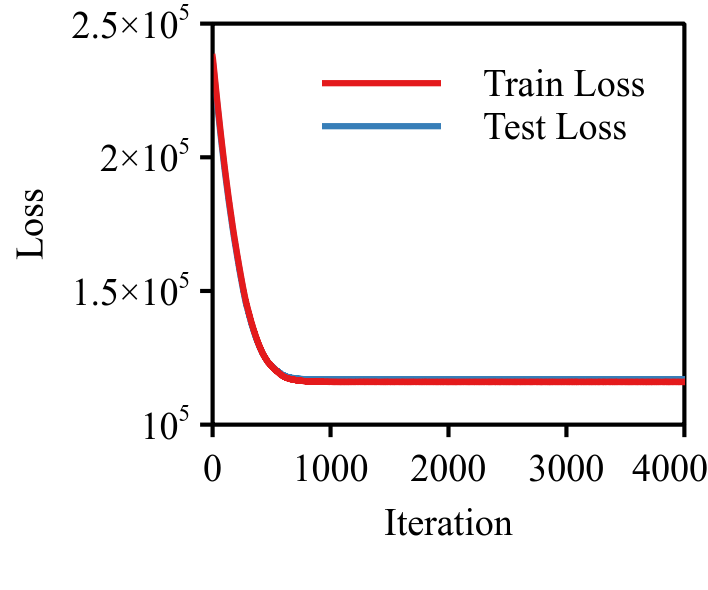
\includegraphics[scale=1.0]{figures/mlp_train_01.png}
  \caption{MLP의 학습 과정.}\label{fig:mlp_train}
\end{figure}
%
MLP는 Figure~\ref{fig:mlp_train}에서 볼 수 있다.
Train loss와 test loss 모두 1000 step 정도에서 수렴을 한 것을 확인할 수 있다.

\begin{figure}[t]
  \centering
  \subfloat[Sample의 값 (trace plot)]{
    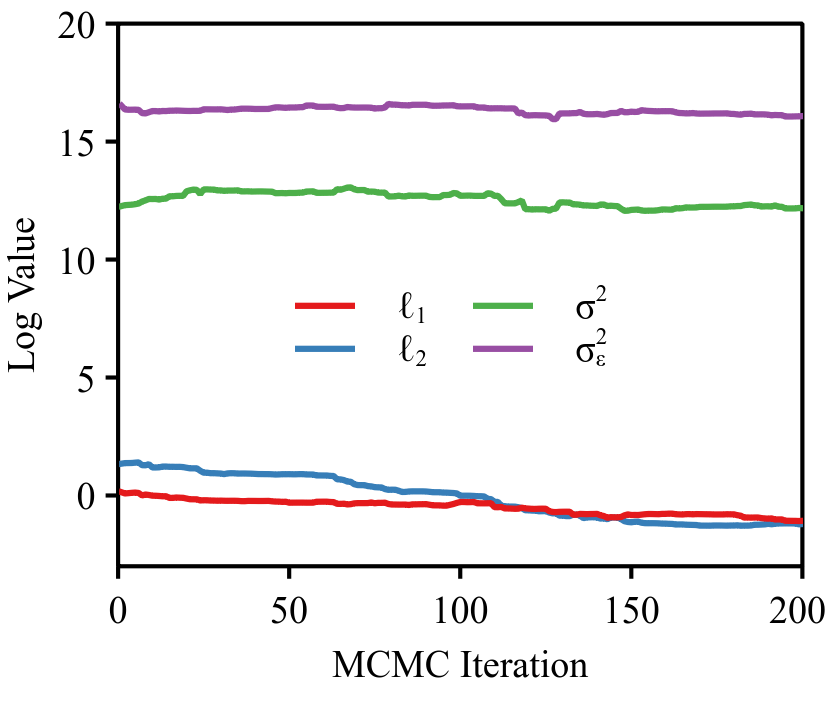
\includegraphics[scale=0.7]{figures/hyper_01.png}
  }
  \subfloat[Autocorrelation]{
    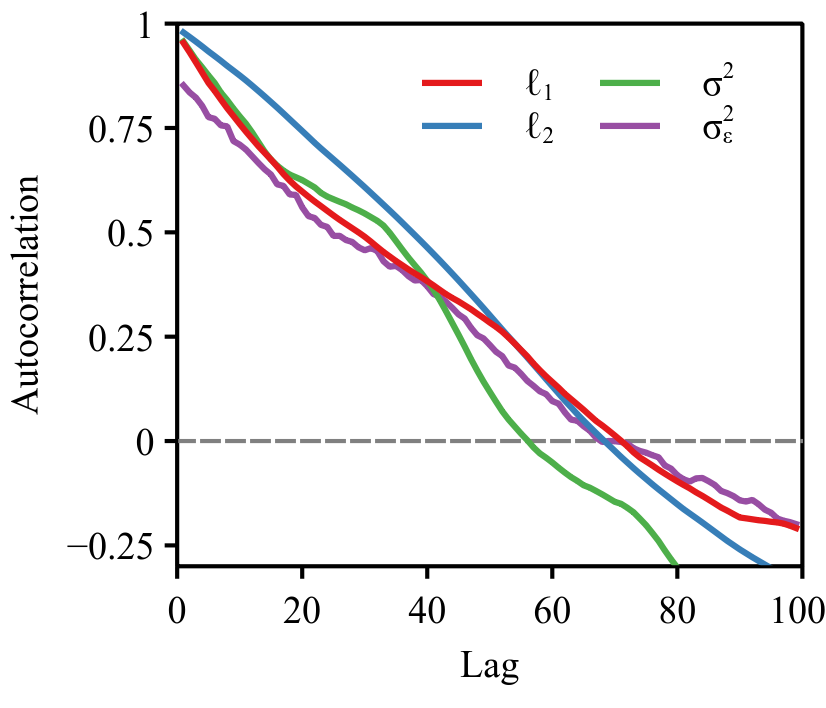
\includegraphics[scale=0.7]{figures/hyper_02.png}\label{fig:autocor}
  }
  \caption{GP 학습 결과.}\label{fig:hyper}
\end{figure}
%
\paragraph{GP training}
GP의 hyperparameter들을 샘플링한 다음, 이 샘플들을 이용해서 prediction을 수행할 수가 있다.
따라서, hyperparameter들을 적절하게 sampling 하는 것이 중요한데, 그 결과를 Figure~\ref{fig:hyper}에서 볼 수 있다.
Hyperparameter들을 샘플링하는 과정에서 수식~\eqref{eq:alpha}을 계산하게 되기 때문에, hyperparameter sampling이 GP의 training을 겸한다고 보면 된다.

MCMC 알고리즘들의 성능 분석은 보통 sample들의 autocorrelation으로 평가하는데~\citep{geyer_practical_1992}, 그것을 Figure~\ref{fig:autocor}에서 볼 수 있다.
Autocorrelation이 0으로 빠르게 수렴할수록 sampling 성능이 좋다는 뜻이다.
Figure~\ref{fig:autocor}의 결과의 경우, autocorrelation이 수렴을 굉장히 늦게 하는 것을 볼 수가 있는데, hyperparmeter들의 sampling 성능이 그다지 좋지 않았던 것으로 보인다.
다만, hyperparameter 샘플들의 통계적 성능이 좋지 않다고 해서 실제 GP의 성능이 나쁘다는 뜻은 아니다.
따라서, 전체 모델의 성능을 확인하기 위해서는 RMSE를 계산해봐야 한다.

\paragraph{성능 평가}
K-fold cross-validation을 수행한 결과를 Table~\ref{table:cv}에서 볼 수 있다.
각 fold 별 RMSE와, 평균 RMSE를 별도로 표기하였다.
결과적으로, MLP에 비해서 GP가 월등히 뛰어난 성능을 보이고 있는 것을 알 수가 있다.

\begin{table*}
  \centering
  \begin{threeparttable}
    \caption{CA Dataset Cross-Validation 결과}\label{table:cv}
    \begin{tabular}{l|rrrrr|r} \toprule
      \multicolumn{1}{c}{\textbf{Method}}
      & \multicolumn{1}{c}{\textbf{Fold 1}}
      & \multicolumn{1}{c}{\textbf{Fold 2}}
      & \multicolumn{1}{c}{\textbf{Fold 3}}
      & \multicolumn{1}{c}{\textbf{Fold 4}}
      & \multicolumn{1}{c}{\textbf{Fold 5}}
      & \multicolumn{1}{c}{\textbf{Average}}
      \\ \midrule
      MLP & 114,027 & 116,850 & 117,282 & 116,483 & 116,044 & 116,137 \\
      GP  & \textbf{46,116}	& \textbf{48,864}  & \textbf{53,973} &  \textbf{48,337}  & \textbf{47,800}  & \textbf{49,018}
      \\ \bottomrule
    \end{tabular}
  \end{threeparttable}
\end{table*}

\paragraph{한계}
GP의 학습 및 예측 성능은 매우 뛰어나다는 것은 알 수 있으나, 한계들이 존재한다.
학습의 경우, 데이터셋에 있는 데이터의 갯수 \(N\)에 대해서 \(\mathcal{O}(N^3)\)만큼의 복잡도를 가진다.
따라서, 큰 데이터셋의 경우 계산량이 굉장히 커지게 된다.
이번 프로젝트의 경우 \(N = 16,000\)정도인데, 계산 시간을 줄이기 위해 GPU를 활용해야 했다.
문제는 GPU를 활용했는데도 fold 1개를 학습하는데 3시간 정도가 소요됐다.
이는 MLP를 batch size 32로 학습 시킬 때 20분 정도가 소요된 것과 비교할 때 매우 긴 시간이다.
GP의 scalability를 극복하기 위해서는 많은 연구들~\citep{hensman_mcmc_2015, yu_stochastic_2017, wang_exact_2019}이 이뤄지고 있다.
미래에 GP의 계산량이 deep learning 기반 방법들과 비슷한 수준으로 내려온다면, 많은 machine learning 문제들이 GP로 해결될 것으로 기대된다.

\bibliographystyle{ba}
\bibliography{references}
\end{document}

